\section{Steep angle analysis}
The background of the portrait images changes together with the pose. Figure \ref{fig:non_rebalanced} shows the input image in the center. All the output images are the surrounding images. When the angle becomes larger, shown in the outermost columns of figure \ref{fig:non_rebalanced}, the extremities of the background turn black. In these same images, the backside of the heads is also distorted with random colors and blurred patches. 
Using a 'rebalanced' model gives much better results, shown in figure \ref{fig:rebalanced}. For the same angles, we can see that the black background and blurring on the rear of the heads have been solved largely. \\
This effect is rather easy to explain. The original model is trained mainly on images where the person looks straight ahead into the camera, such as the middle (input) picture in figures \ref{fig:non_rebalanced} and \ref{fig:rebalanced}. This means that the model has less knowledge about side projections of human heads, what the back of the head looks like and changes in background features. \\
The rebalanced model has a more uniformly distributed training dataset \cite{github}. By comparison,  rebalanced network has more training images where the person has an angle with respect to the camera. Therefore, this model knows the features on the side and rear of the head better than the original model. Additionally, it can learn about changes in background features. This explains why the rebalanced model can extrapolate the colors of the background better, and why the backsides of the heads are no longer blurred.
\begin{figure}[H]
\centering
  \centering
  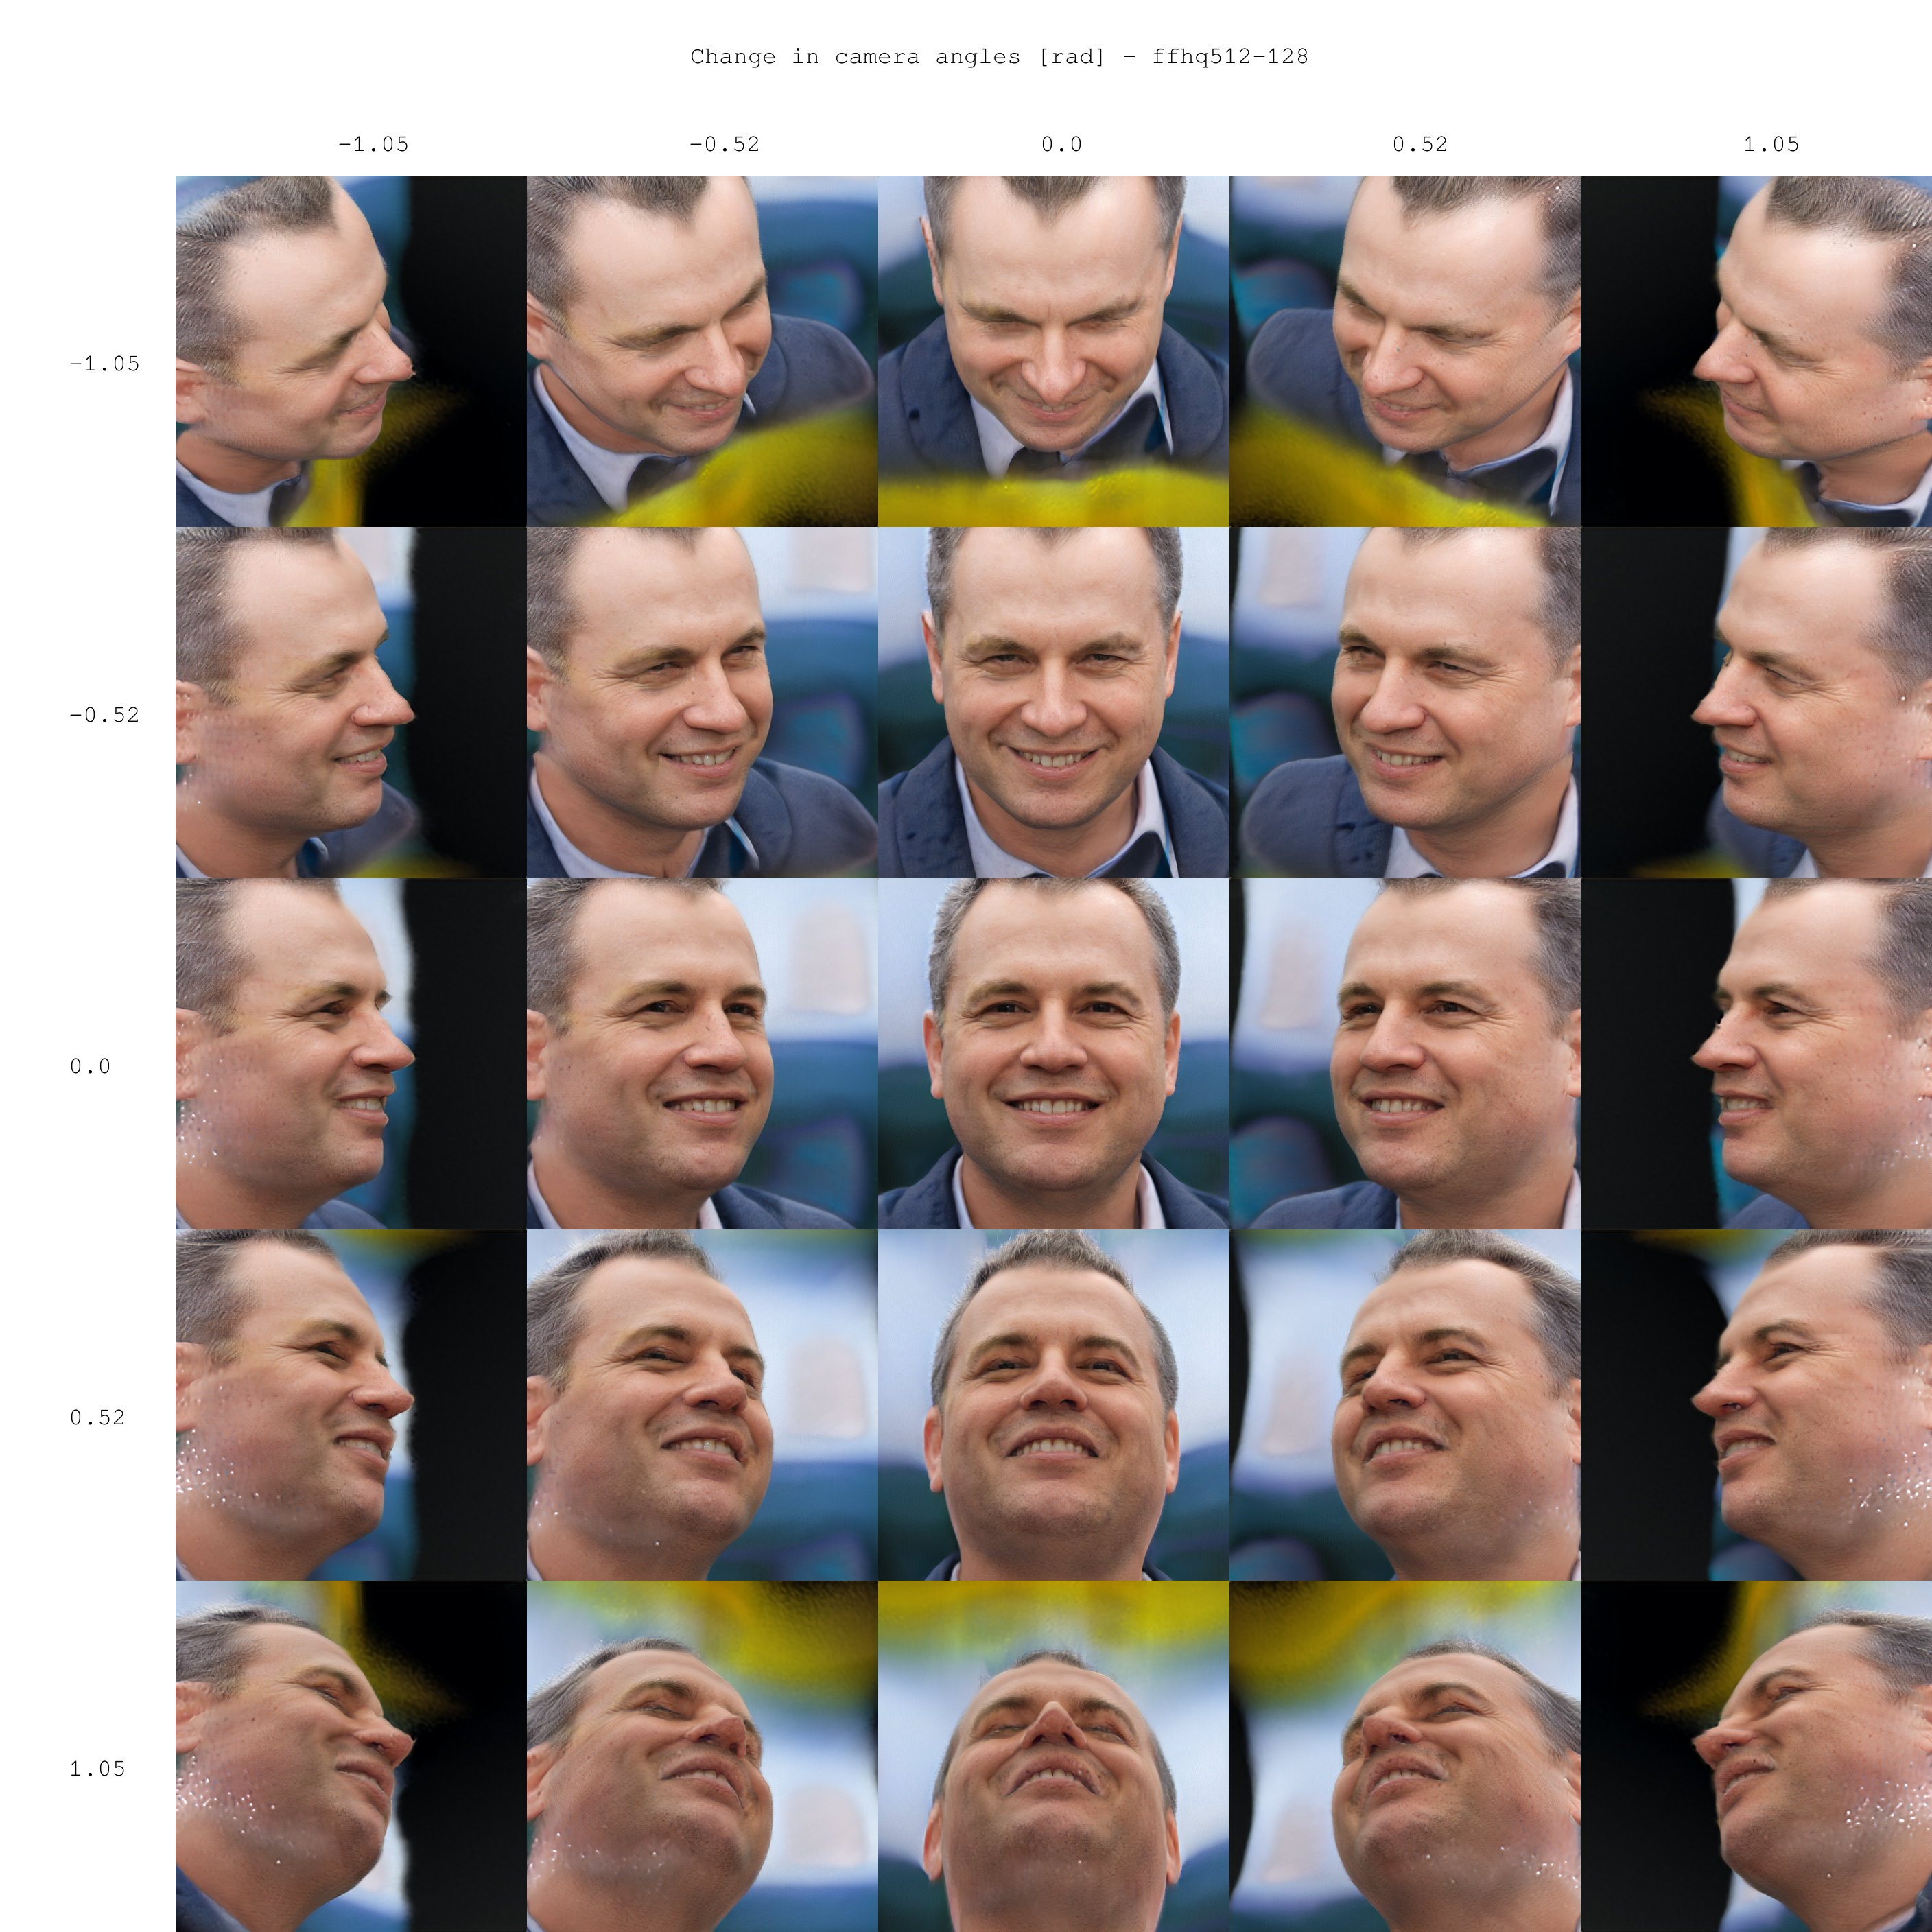
\includegraphics[width=0.6\linewidth]{angles-0001-ffhq512-128.png}
  \caption{Background with black patches using original model}
  \label{fig:non_rebalanced}
\end{figure}
\begin{figure}[H]
  \centering 
  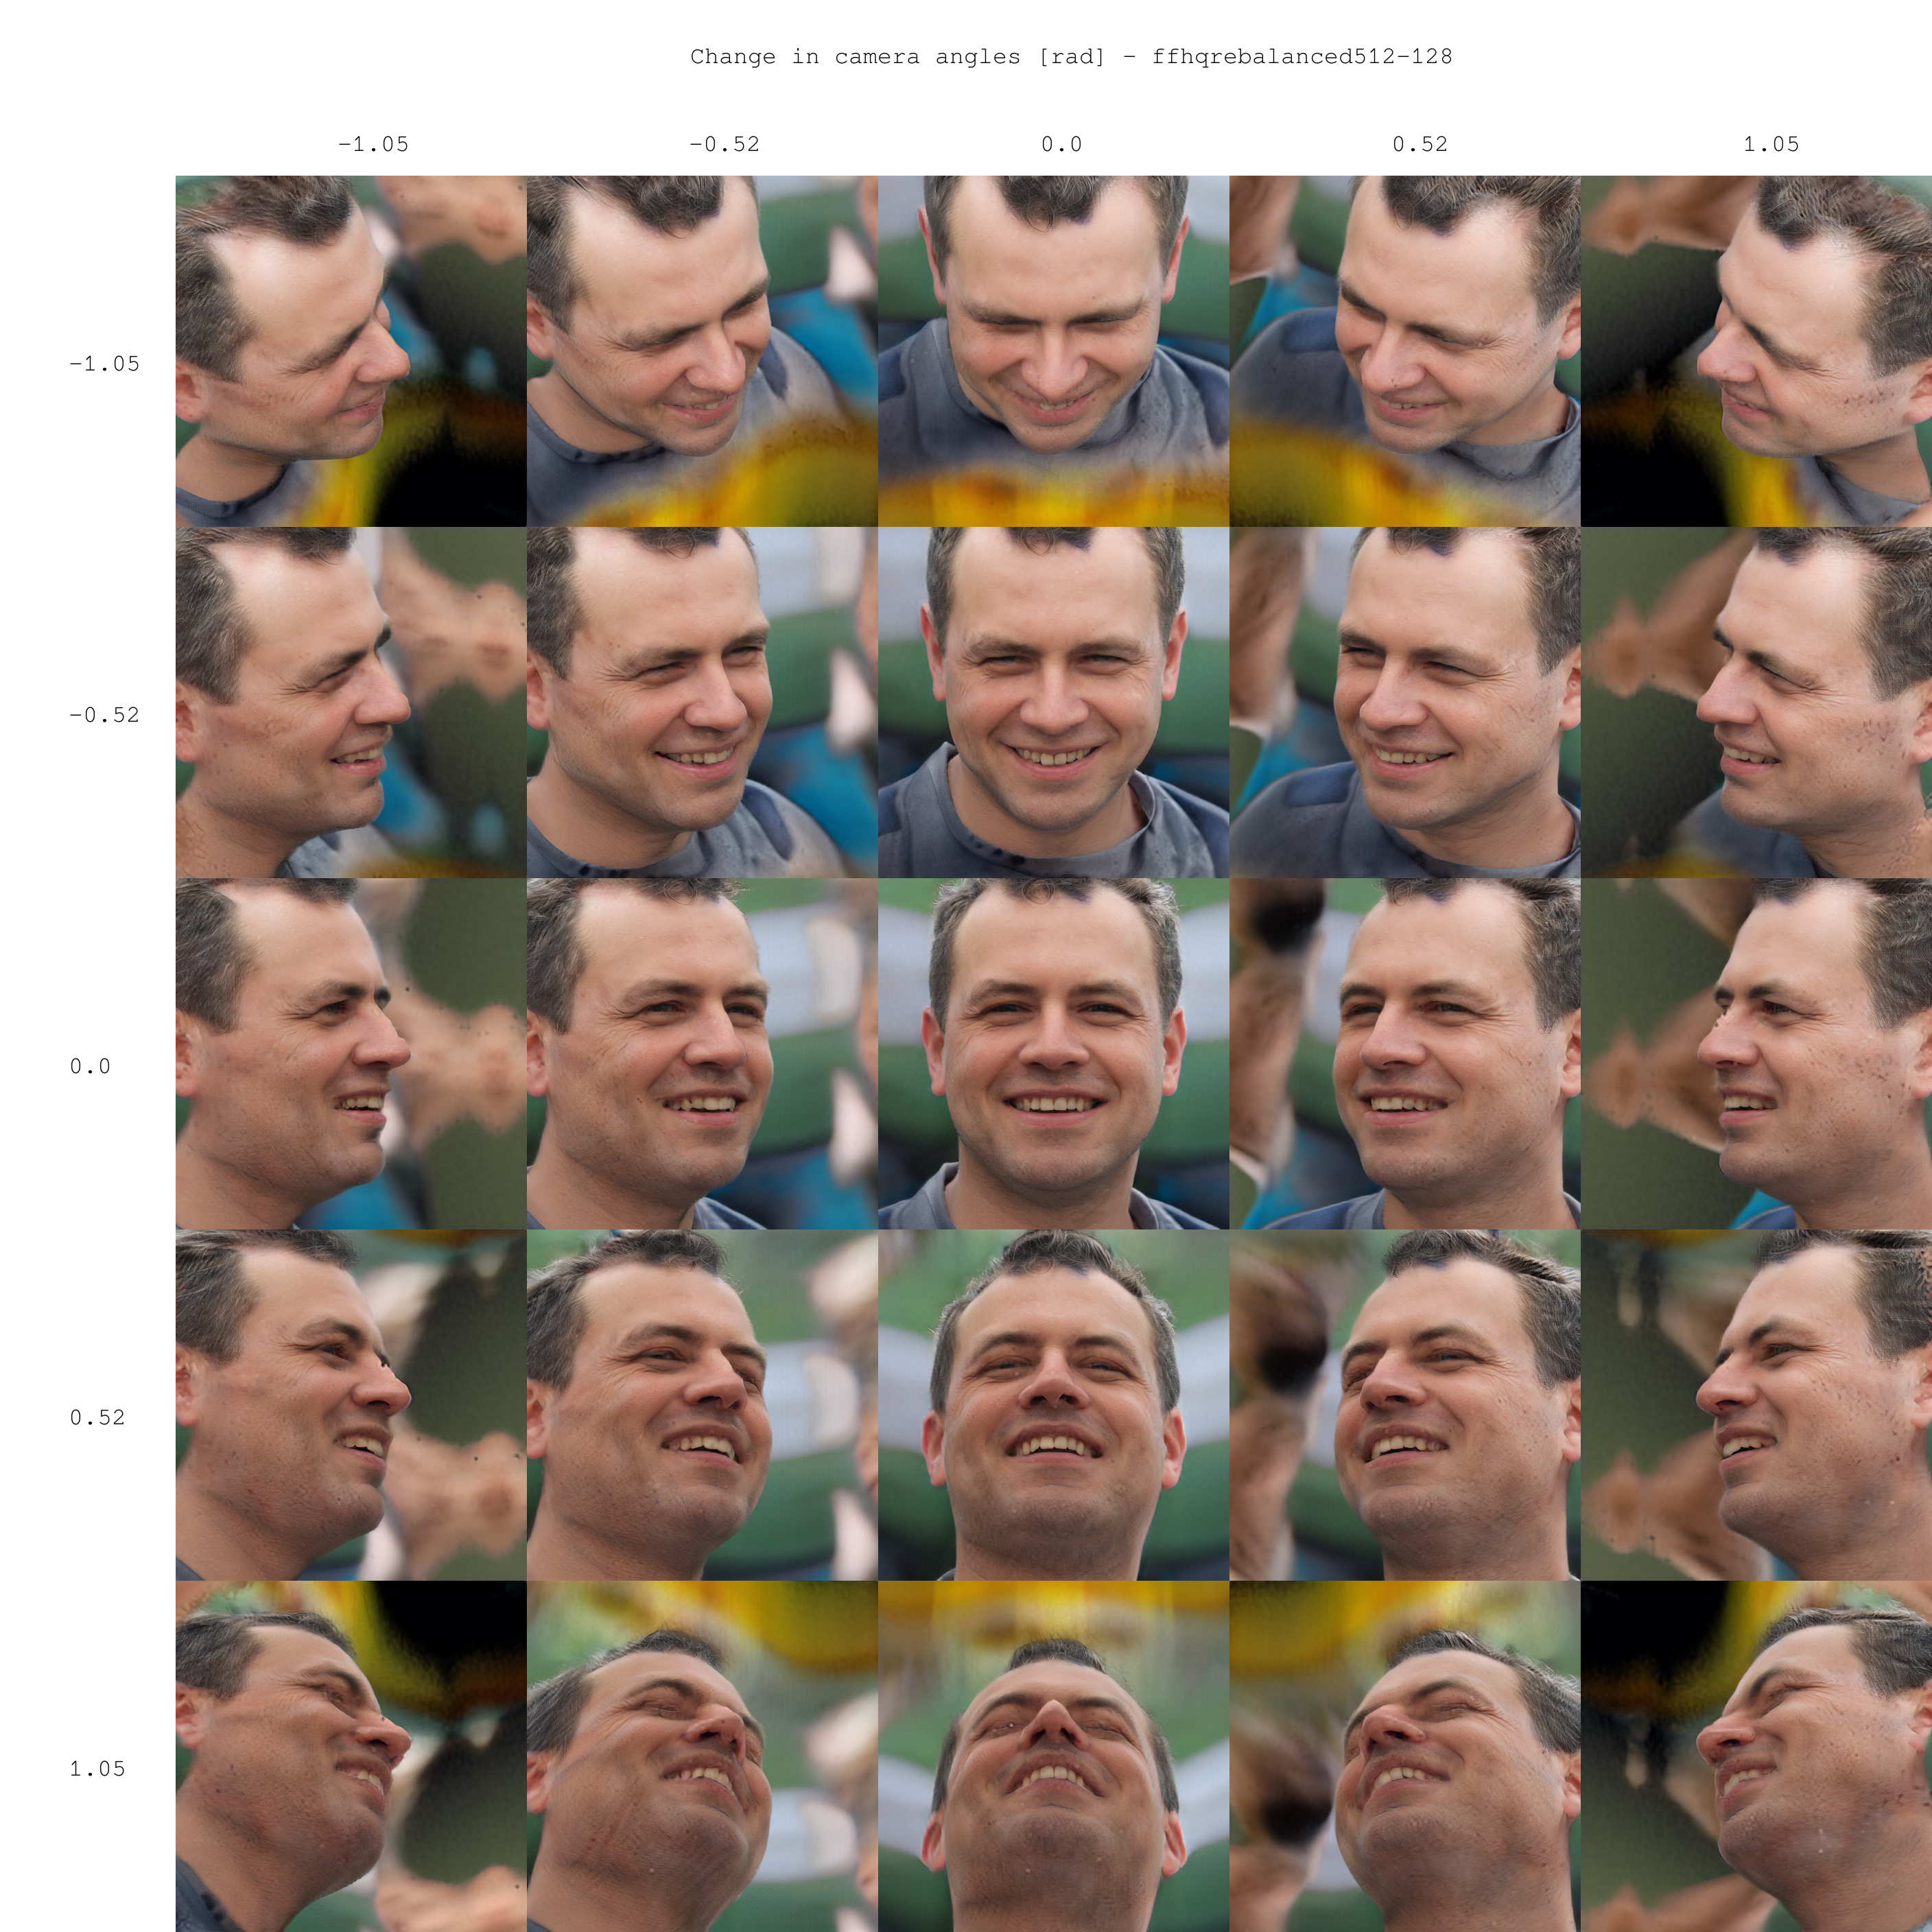
\includegraphics[width=0.6\linewidth]{angles-0001-ffhqrebalanced512-128.png}
  \caption{Background improvements using rebalanced model}
  \label{fig:rebalanced}
\end{figure}
To provide further evidence, we studied the neural volume renderer of the model to see how values of color and density cause the final rendered image to be dark where little knowledge is available. Figures \ref{fig:density_seed1} and \ref{fig:color_seed1} show the values of density and colour that are the output of the tri-plane, and are used by "volume rendering" to create the raw image. For the dark regions, we can see that the colours values are close to black, and densities are close to zero. Low volume density values particularly signify that there is no surface on which the ray will terminate. At the right side (near the back of the head) of figure \ref{fig:seed1_extreme_angle}, we see that volume density is high - correctly -, but presumably because of absence of any knowledge, the color values are unknown, and therefore close to zero (i.e. black). Together this analysis explains why the extremities of renders become black in very oblique angles.

\begin{figure}[H]
    \centering
    \includegraphics[width=0.5\linewidth]{seed0001.png}
    \caption{Rendered image with black background in the border}
    \label{fig:seed1_extreme_angle}
\end{figure}

\begin{figure}[H]
    \centering
    \includegraphics{test1blog.png}
    \caption{Variation of density values across channels. First three images are of channels equidistant from each other with the rightmost image being an average value of all channels.}
    \label{fig:density_seed1}
\end{figure}

\begin{figure}[H]
    \centering
    \includegraphics{test1cblog.png}
    \caption{Variation of color values across channels. 32 channel feature-images are output, only the first three channels are rendered}
    \label{fig:color_seed1}
\end{figure}